\documentclass[english,14pt]{beamer}
\usetheme{EastLansing}
\usecolortheme{spruce}

\usepackage{xcolor}
\usepackage{listings}
\usepackage{courier}
\usepackage{graphicx}
\usepackage{amsmath}
\usepackage{algorithm2e}
\usepackage{multicol}
\usepackage{hyperref}

% http://mirrors.ibiblio.org/CTAN/macros/latex/contrib/datetime2/datetime2.pdf
\usepackage{babel}
\usepackage[useregional]{datetime2}

% https://tex.stackexchange.com/questions/42619/x-mark-to-match-checkmark
\usepackage{pifont}% http://ctan.org/pkg/pifont

%% https://stackoverflow.com/questions/1435837/how-to-remove-footers-of-latex-beamer-templates
%%gets rid of bottom navigation bars
%\setbeamertemplate{footline}[page number]
%
%gets rid of navigation symbols
\setbeamertemplate{navigation symbols}{}


\usefonttheme[onlymath]{serif}

\definecolor{mGreen}{rgb}{0,0.6,0}
\definecolor{mGray}{rgb}{0.5,0.5,0.5}
\definecolor{mPurple}{rgb}{0.8,0,0.82}
\definecolor{backgroundColour}{rgb}{0.95,0.95,0.92}
\definecolor{lightBlue}{rgb}{0.1, 0.1, 0.8}

\newcommand\red[1]{{\color{red} #1}}
\newcommand\green[1]{{\color{green} #1}}
\newcommand\blue[1]{{\color{blue} #1}}

\newcommand{\cmark}{\ding{51}}%
\newcommand{\xmark}{\ding{55}}%

\lstdefinestyle{CStyle}{
    backgroundcolor=\color{backgroundColour},   
    commentstyle=\color{mGreen},
    keywordstyle=\color{magenta},
    numberstyle=\tiny\color{mGray},
    stringstyle=\color{mPurple},
    basicstyle=\footnotesize,
    breakatwhitespace=false,         
    breaklines=true,                 
    captionpos=b,                    
    keepspaces=true,                 
    numbers=left,                    
    numbersep=5pt,                  
    showspaces=false,                
    showstringspaces=false,
    showtabs=false,                  
    tabsize=2,
    language=C
}

\lstdefinestyle{pseudo}{
        basicstyle=\ttfamily\footnotesize,
        keywordstyle=\color{lightBlue},
        morekeywords={BEGIN,END,IF,ELSE,ENDIF,ELSEIF,PRINT,WHILE,RETURN,ENDWHILE,DO,FOR,TO,IN,ENDFOR,BREAK,INPUT},
        morecomment=[l]{//},
        commentstyle=\color{mGreen}
}

\lstset{basicstyle=\footnotesize\ttfamily,breaklines=true}
\lstset{framextopmargin=50pt,tabsize=2}

\title{ENGG1003 - Monday Week 8}
\subtitle{Solving nonlinear algebraic equations }%\\ \& computing integrals}
\author{Steve Weller}
\institute{University of Newcastle}
%\date{\today}
\date{26 April 2021}

% following is a bit of a hack, but forces page numbers (technically: frame numbers) to run 1,2,3,... 
% with titlepage counting as frame 1

\addtocounter{framenumber}{1}
\titlepage

\begin{document}

\begin{flushleft}
{\scriptsize Last compiled:~\DTMnow}
\vspace*{-5mm}
\end{flushleft}
\framebreak

%==============================================================

\begin{frame}[fragile]

\frametitle{Lecture overview}
\begin{enumerate}
	\item Solving nonlinear algebraic equations \red{pp.~175-176}
	\begin{itemize}
		\item general setting
		\item two problems: flight time, fluid level
	\end{itemize}
	
	\item[]
	
	\item Bisection method \red{\S7.4}
	
	\item[]
	
	\item Secant method \red{\S7.3}
	\begin{itemize}
		\item Newton--Raphson method
	\end{itemize}
	
	\item[]
	
	\item Extensions
	\begin{itemize}
		\item bisection \& secant methods: re-write as functions
		\item timing code in Python
		\item speed comparisons
%		\item initialisation \& failure to converge
	\end{itemize}
	
\end{enumerate}

\end{frame}

%==============================================================

\begin{frame}[fragile]

\frametitle{$1)$ Solving nonlinear algebraic equations}

\begin{itemize}
	\item \red{\emph{linear}} equations: $ax + b = 0$
	\begin{itemize}
		\item solution $x = -b/a$
	\end{itemize}
	\item[]
	\item \red{\emph{nonlinear}} equations
	\begin{itemize}
		\item quadratic $ax^2 + bx+c = 0$: solution $x = \frac{-b \pm\sqrt{b^2-4ac}}{2a}$
		\item cubic and quartic (orders $3$ and $4$): exact solutions exist but are \emph{very} complicated
		\item quintic (order $5$) equations: exact solutions \emph{do not exist} in general, proving that needs \emph{serious} mathematics
	\end{itemize}
	\item[]
	\item most equations in engineering applications have no exact ``pen and paper'' solutions!
	
	
\end{itemize}

\end{frame}

%==============================================================

\begin{frame}[fragile]

\frametitle{Numerical solutions to equations}

\begin{flushright}
\small \emph{``An approximate answer to the right problem is worth a good deal more than an exact answer to an approximate problem''\\ ---John Tukey}
\end{flushright}
\vspace*{-3mm}
\textbf{General problem:} find $x$ satisfying
	\[
		f(x) = 0
	\]
	where $f(x)$ is a formula involving $x$
	
	\textbf{Example}
	\[
		f(x) = e^{-x}\sin(x) - \cos(x)
	\]
	has solution $x = 7.85359326$ because
	\[
	e^{-7.85359326}\sin(7.85359326) - \cos(7.85359326) = 0.00
	\]

\end{frame}

%==============================================================

\begin{frame}[fragile]

\frametitle{Flight time}

\begin{itemize}
	\item one more time!
\end{itemize}

\end{frame}

%==============================================================

\begin{frame}[fragile]

\frametitle{Fluid level}

image of measuring cup

\begin{figure}[ht]
	\centering
	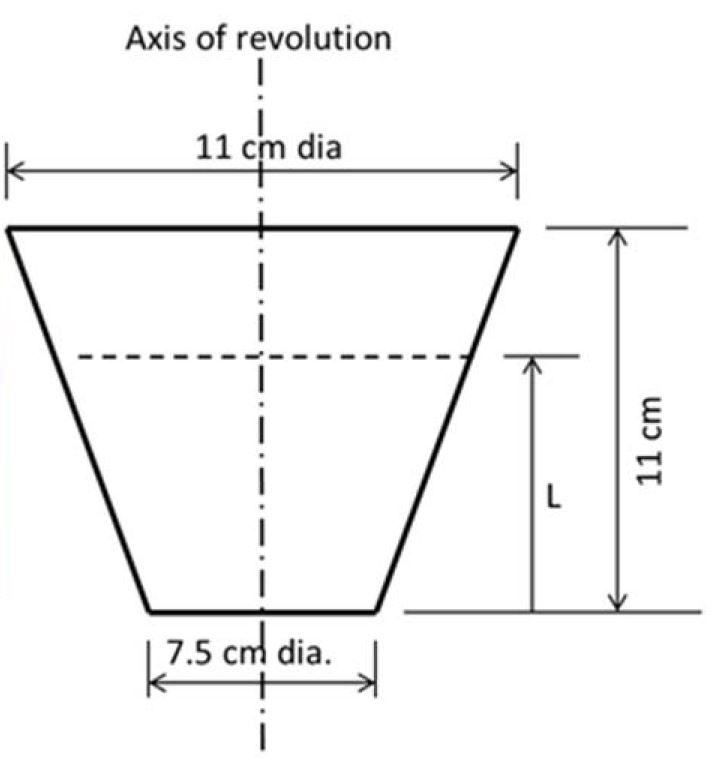
\includegraphics[width=0.5\textwidth]{figures/cupDimensions}
\end{figure}

\end{frame}

%==============================================================

\begin{frame}[fragile]

\frametitle{Fluid level}

% https://www.sjsu.edu/me/docs/hsu-Chapter%2010%20Numerical%20solution%20methods.pdf
% Section 10.3.2

\begin{itemize}
	\item cup dimension figure
	\item water in dam, coal in stockpile
	\item volume $V$ (mL) depends on depth $L$ as follows, \emph{presented without proof:}
	\[
		V = 0.0268L^3 + 1.884L^2 + 44.15L
	\]
	\item Question: depth $L$ when cup holds $500$~mL of water?
	\item solve $f(L) = 0$ where
	\[
		F(L) = 0.0268L^3 + 1.884L^2 + 44.15L - 500
	\]
\end{itemize}

\end{frame}

%==============================================================

\begin{frame}[fragile]

\frametitle{$2)$ Bisection method}

\begin{itemize}
	\item basic idea: visualisation
\end{itemize}

\end{frame}

%==============================================================

\begin{frame}[fragile]

\frametitle{}

\begin{itemize}
	\item bisection method: key equations
\end{itemize}

\end{frame}

%==============================================================

\begin{frame}[fragile]

\frametitle{}

\begin{itemize}
	\item bisection method: pseudocode
\end{itemize}

\end{frame}

%==============================================================

\begin{frame}[fragile]

\frametitle{}

\begin{itemize}
	\item bisection method: Python code
	\item live demo
\end{itemize}

\end{frame}

%==============================================================

\begin{frame}[fragile]

\frametitle{}

\begin{itemize}
	\item bisection method: simulation results
\end{itemize}

\end{frame}

%==============================================================

\begin{frame}[fragile]

\frametitle{$3)$ Secant method}

\begin{itemize}
	\item basic idea: visualisation
\end{itemize}

\end{frame}

%==============================================================

\begin{frame}[fragile]

\frametitle{}

\begin{itemize}
	\item secant method: key equations
\end{itemize}

\end{frame}

%==============================================================

\begin{frame}[fragile]

\frametitle{}

\begin{itemize}
	\item secant method: pseudocode
\end{itemize}

\end{frame}

%==============================================================

\begin{frame}[fragile]

\frametitle{}

\begin{itemize}
	\item secant method: Python code
	\item live demo
\end{itemize}

\end{frame}

%==============================================================

\begin{frame}[fragile]

\frametitle{}

\begin{itemize}
	\item secant method: simulation results
\end{itemize}

\end{frame}

%==============================================================

\begin{frame}[fragile]

\frametitle{Newton--Raphson method}

\begin{itemize}
	\item xxx
\end{itemize}

\end{frame}

%==============================================================

\begin{frame}[fragile]

\frametitle{$4)$ Extensions: re-write methods as functions}

\begin{itemize}
	\item bisection re-write as function
\end{itemize}		

\end{frame}

%==============================================================

\begin{frame}[fragile]

\frametitle{}

\begin{itemize}
	\item secant re-write as function
\end{itemize}		

\end{frame}

%==============================================================

\begin{frame}[fragile]

\frametitle{Timing code in Python}

\begin{itemize}
	\item import time
	\item \verb+tStart = time.perf_counter()+
	\item (code)
	\item \verb+tStop = time.perf_counter()+
	\item elapsedTime = tStop-tStart
\end{itemize}

\end{frame}

%==============================================================

\begin{frame}[fragile]

\frametitle{Speed comparisons: bisection vs.~secant}

\begin{itemize}
	\item xxx
	\item xxx
\end{itemize}

\end{frame}

%%==============================================================
%
%\begin{frame}[fragile]
%
%\frametitle{}
%
%\begin{itemize}
%	\item initialisation
%	\item failure to converge
%\end{itemize}
%
%\end{frame}

%==============================================================

\begin{frame}[fragile]

\frametitle{Lecture summary}
\begin{itemize}
	\item Solving nonlinear algebraic equations

	\item[]
	
	\item Bisection method

	\item[]
	
	\item Secant method
	\begin{itemize}
		\item Newton--Raphson method
	\end{itemize}

	\item[]
	
	\item Extensions
	
\end{itemize}

\end{frame}

%==============================================================

\begin{frame}[fragile]

\frametitle{More information}
\begin{itemize}
	\item Newton--Raphson method in \red{\S7.2} textbook
	\begin{itemize}
		\item known as Newton's method
		\item needs differential calculus MATH1110
	\end{itemize}
	\item[]
	
	\item \red{\S7.3} and \red{\S7.4 }text for ``optimised'' versions of bisection and secant methods, which minimise number of function calls

	\item[]
	
	\item extension: proof of measuring cup volume \verb+https://www.sjsu.edu/me/docs/hsu-Chapter\%2010\%20Numerical\%20solution\%20methods.pdf+
	
\end{itemize}

\end{frame}

\end{document}